\documentclass[conference]{IEEEtran}
\IEEEoverridecommandlockouts
% The preceding line is only needed to identify funding in the first footnote. If that is unneeded, please comment it out.
\usepackage{cite}
\usepackage{amsmath,amssymb,amsfonts}
\usepackage{algorithmic}
\usepackage{graphicx}
\usepackage{textcomp}
\usepackage{xcolor}

%my pacakges
%\usepackage{mymacros}

%\usepackage{xspace}

%%
\usepackage[colorlinks=true,urlcolor=blue,citecolor=blue]{hyperref}
\usepackage{url}
\usepackage{xspace}
\usepackage{todonotes}

\usepackage{subcaption}
\usepackage{graphicx}
\usepackage{multicol}
\usepackage{cleveref}

% theorems
\newtheorem{example}{Example}[section]




%% macros
\newcommand{\abaddrule}{\texttt{aba-dd-rule-based}\xspace}
\newcommand{\flexable}{\texttt{flexABle}\xspace}
\newcommand{\abagraph}{\texttt{abagraph}\xspace}
\newcommand{\scala}{\texttt{Scala}\xspace}

\newcommand{\iccma}{ICCMA 2023}

\newcommand{\frF}{\ensuremath{\mathcal{F}}\xspace}
\newcommand{\frL}{\ensuremath{\mathcal{L}}\xspace}
\newcommand{\frA}{\ensuremath{\mathcal{A}}\xspace}
\newcommand{\frCtr}{\ensuremath{\overline{\phantom{x}}}\xspace}
\newcommand{\frR}{\ensuremath{\mathcal{R}}\xspace}
\newcommand{\frTup}{\ensuremath{(\frL,\frA,\frCtr,\frR)}\xspace}
\newcommand{\fr}{\ensuremath{\frF = \frTup}\xspace}

\newcommand{\rulH}{\ensuremath{h}\xspace}
\newcommand{\rulB}{\ensuremath{B}\xspace}
\newcommand{\rul}{\ensuremath{\rulH \leftarrow \rulB}\xspace}

\newcommand{\rulA}[2]{\ensuremath{#1 \leftarrow #2}\xspace}
\newcommand{\argu}[1]{\ensuremath{A_{#1}}}
\newcommand{\arguInline}[2]{\ensuremath{[\rulA{#1}{#2}]}}
\newcommand{\stmt}[1]{\ensuremath{#1}}

\def\BibTeX{{\rm B\kern-.05em{\sc i\kern-.025em b}\kern-.08em
    T\kern-.1667em\lower.7ex\hbox{E}\kern-.125emX}}
\begin{document}

\title{\flexable -- System Description for \iccma
  \thanks{The authors are funded by the German Federal Ministry of Education and Research (BMBF) via the Center for Scalable Data Analytics and Artificial Intelligence (ScaDS.AI), project 13GW0552B (KIMEDS, KI-assistierte Zertifizierung medizinischer Software), and grant  01IS20056\_NAVAS respectively.     }
}


\author{
\IEEEauthorblockN{Martin Diller}
\IEEEauthorblockA{\textit{Logic Programming} \\ \textit{and Argumentation Group} \\
\textit{TU Dresden, Germany}\\
martin.diller@tu-dresden.de}
\and    
\IEEEauthorblockN{Sarah Alice Gaggl }
\IEEEauthorblockA{\textit{Logic Programming} \\ \textit{and Argumentation Group} \\\textit{TU Dresden, Germany}\\
sarah.gaggl@tu-dresden.de}
\and
\IEEEauthorblockN{Piotr Gorczyca}
\IEEEauthorblockA{\textit{Computational Logic Group} \\
\textit{TU Dresden, Germany}\\
piotr.gorczyca@tu-dresden.de}
}





\maketitle

\begin{abstract} We describe \flexable, a system for (interactively \& automatically) computing dialectical justifications of claims in assumption-based argumentation or ABA.  The system participates in the \iccma~ABA tracks for determining credulous acceptance of claims for the complete and stable semantics.      
\end{abstract}

\begin{IEEEkeywords}
argumentation competition, assumption-based argumentation, dispute derivations, explanation
\end{IEEEkeywords}


\section{Introduction}
Dispute derivations~\cite{Toni13,CravenT16,DillerGG21} %\cite{DungKT06,DungMT07,GaertnerT08,Toni13,CravenTW13,CravenT16}
are one of the main native %(vs. reduction-based as in e.g.~\cite{LehtonenWJ21}) %~\cite{CeruttiGTW18,LehtonenWJ21})
reasoning methods for assumption-based argumentation or ABA~\cite{%BondarenkoTK93,BondarenkoDKT97,DungKT09,
  %Toni14%,
  CyrasFST18
}\footnote{More concretely, flat propositional Horn-ABA.%~\cite{CyrasHT21}.
}.  Based on games for abstract argumentation~\cite{Caminada18}, %; namely, argumentation games (see e.g.~\cite{JakobovitsV99,PrakkenS97,DoutreM04,VreeswijkP00,ModgilC09,ThangDH09,Caminada15,Caminada18,0001CM18,ZafarghandiVV19,ZafarghandiVV20}).
they are conceived of as a dispute with arguments for and against some claims under scrutiny being exchanged by a proponent and an opponent of the claims.  The arguments themselves are proof trees: they consist of a claim (the conclusion) derived from assumptions (uncertain premisses) and facts (certain premisses) via chaining of rules (modus ponens).  More than just a method for reasoning about acceptance of claims, they provide a means of dialectical explication~\cite{Cyras0ABT21}.  %Concretely, such a justification consists not only of initial arguments for the claims but also relevant counter-arguments to such arguments, together with further arguments defending the initial arguments from the counter-arguments, and so on.
%Nevertheless, in contrast to games for abstract argumentation, for their unfolding disputes for ABA take in account, not only the attack relation of arguments, but also their structure; thus, for instance, arguments put forward by the opponent need not be completely constructed before they can be attacked by the proponent, and arguments making use of assumptions which have already been attacked by the proponent can be disregarded for further attacks.          

%, where starting from some goal claim the proponent searches for an argument proving the goal.  This search reveals assumptions on which the argument depends, which can be attacked by the opponent by arguments for their contraries.  Such arguments from the opponent can in turn be attacked by the proponent by further arguments and so on.%  Dispute derivations can be seen as hybrid syntactic-semantic methods for searching for only those arguments needed to answer a query and are thus related to the issue of selecting such relevant arguments in structured argumentation more general (see \eg~\cite{%EfstathiouH11,AmgoudBV14,
%  BorgS18,StrassWD19,ThimmR20,YunOC20}).  %In the context of ABA for this reason
% They can for this reason also be the basis of argumentation-based explanations for acceptance of claims (see \eg~\cite{GarciaCRS13,FanT15,BorgB21b} for relevant notions mainly in abstract argumentation).  Moreover, dispute derivations are quite natural to use in an interactive setting, for keeping human users in the loop           
%Although reduction-based methods for reasoning in ABA have to date proved to be more efficient than dispute derivations~\cite{LehtonenWJ21},
%~\cite{LehtonenWJ17,LehtonenWJ19}
%dispute derivations remain interesting for a number of reasons.  The main of these is that they allow for a dialectic evaluation of claims in terms of arguments and counter-arguments.  This means, first of all, that dispute derivations deliver ``dialectic explications'' for acceptance of claims; these can, in turn, underly the afore-mentioned more sophisticated forms of dialectical explanation.  Related to this, dispute derivations are %, in contrast to the available reduction-based methods,
%quite natural to use in an interactive setting in which human users are to be kept in the loop.  Moreover, dispute derivations are quite general procedures and are promising to investigate further in direction of supporting more expressive forms of argumentation as well as the basis for truly dynamic argument-based reasoning (see \eg~\cite{FanT14}).


The system \flexable implements flexible dispute derivations for ABA~\cite{DillerGG21}; these build on previous forms of dispute derivations~\cite{Toni13,CravenT16}, while also differing in the following substantial aspects:

\begin{itemize}
\item In flexible dispute derivations the proponent and opponent are completely omniscient in that they remember all arguments (and sub-arguments) put forward during a dispute; this avoids redundancy in the sense that repetition of arguments is avoided.    
\item Related to the above, flexible disputes are defined in both an argumentation-based as well as a rule-based version.  In the first, at each move, the proponent and opponent start the construction of new arguments to the dispute (by putting forward assumptions or facts), or expand arguments which already form part of an ongoing dispute (by making use of a rule).  In the second, implementation-oriented representation (in that arguments do not need to be explicitly constructed or stored), dispute states consist simply in the set of claims and rules which have been put forward up until that state and a move consists in adding a new claim or rule to this set.   To the extent that the rule-based representation includes also information about the relationships between claims and rules, it can also be thought of as operating on a graph.  In this aspect flexible disputes take graph-based disputes~\cite{CravenT16} one step further: all arguments put forward in a dispute are represented as a graph and not only those of the proponent.
\item In addition to backward moves (or top-down, from claims to premisses) as in previous versions of disputes, flexible disputes also allow forward (or bottom-up) moves.  Specifically, new assumptions can be added to disputes and claims derived by deducing them from claims previously put forward.  This often leads to shorter disputes for deciding acceptance of claims wrt the admissible (and, hence, complete) semantics (notably in that the proponent can deduce further claims from the assumptions it has commited to and, thus, preemptively block further lines of attack from the opponent). Moreover, via forward moves, variants of disputes can be defined not only for deciding acceptance, but also finding complete and stable assumption sets congruous with the goal claims.
\item Finally, flexible dispute derivations are also more flexible in the flexibility of moves allowed at each step.  In particular, if Dung's abstract argumentation frameworks are encoded as ABA frameworks, then via flexible disputes one obtains games for deciding acceptance of arguments that are not dispute-tree-based~\cite{Caminada18}.
\end{itemize}


\section{An example}

%\begin{example}\label{ex:framework}
% Find out whether $s$ is credulously acceptable under the complete (admissible) semantics in .
%\end{example}


Consider the ABA framework \fr, with assumptions $\frA = \{ a,b,c,d,e,f,g,h \}$, contrary relation $\frCtr(\alpha) = \bar{\alpha}$ for $\alpha \in \frA$ and rules $\frR = \{ \rulA{s}{a,f,\bar{g}}; \rulA{\bar{g}}{b,u}; \rulA{u}{d}; \rulA{\bar{f}}{g,w}; \rulA{w}{e};\rulA{\bar{a}}{c,\bar{g}};\rulA{\bar{c}}{h,u};\rulA{\bar{c}}{u};\rulA{\bar{h}}{y,z} \}$.  The underlying langauge of \fr is $\frL = \frA \cup \bigcup_{\rul \in \frR} \{ \rulH \} \cup \rulB$. 
%\big\{ \{ \rulH \} \cup \rulB  \mid  \rul \in \frR \big\}$.

The argument-based representation of a flexible dispute that shows credulous acceptance of $s$ for the admissible (and complete) semantics is shown in Figure~\ref{fig:diagrams}. To obtain this dispute the proponent first performs three (conservative) backward moves from the goal $s$ using rules 1) $\rulA{s}{a,f,\bar{g}}$, 2) $\rulA{\bar{g}}{b,u}$, and  3) $\rulA{u}{d}$. Thus the proponent has a complete argument for $s$, argument $A_1$ in the figure; i.e. one in which the premisses are all assumptions (or facts) (the piecewise construction of $A_1$ being shown via the boxes with dashed lines labelled $0$, $1$, $2$, $3$).  Now the opponent moves (non-conservatively) backward one step only by making use of the rule 4) $\rulA{\bar{a}}{c,\bar{g}}$ attacking assumption $a$ of argument $A_1$.  Immediately the complete argument $A_2$ attacking $A_1$ in the Figure becomes part of the dispute, since a sub-argument supporting $\bar{g}$ has already been put forward (a sub-argument of $A_1$).  There are no further arguments attacking $A_1$ that can be put forward by the opponent, since the other rule supporting a contrary of an assumption appearing in $A_1$ ($\rulA{\bar{f}}{g,w}$) is blocked in virtue of the proponent already having an argument questioning assumption $g$ (the sub-argument of $A_1$ with conclusion $\bar{g}$).  Now the proponent could try to attack $A_2$ by exploring argument lines against the assumption $c$ making use of either rules $\rulA{\bar{c}}{h,u}$ or $\rulA{\bar{c}}{u}$, but there is no need to guess if rather the proponent makes one (conservative) forward move deriving $\bar{c}$ from the sub-argument of $A_1$ concluding $u$ by making use of the rule 5) $\rulA{\bar{c}}{u}$ (argument $A_3$ in the figure). In fact, if the proponent would have followed a more eager strategy and constructed $A_3$ right after $A_1$ then the dispute would have ended there (in four steps rather than five), since this move would have preemptively blocked the rule $\rulA{\bar{a}}{c,\bar{g}}$ and thus the construction of the opponent's argument $A_2$.   






%The credulous acceptance of $s$ can be proven with merely 5 moves of the FlexDDs game, i.e.:
%  \begin{enumerate}
%    \renewcommand{\labelenumi}{step \arabic{enumi}.}
%    \item P: \rulA{s}{a,f,\bar{g}}
%    \item P: \rulA{\bar{g}}{b,u}
%    \item P: \rulA{\bar{u}}{d}
%    \item P: \rulA{\bar{c}}{u}
%    \item O: \rulA{\bar{a}}{v,\bar{g}}
%  \end{enumerate}
%Explanation
%\begin{itemize}
%    \item steps 1-3 is just backward expansion of \stmt{s} 
%    \item step 4 is a forward move - reuses a complete argument \arguInline{u}{d}, this rule does not have to be repeated
%    \item item step 5 is an attack on the defence \stmt{a}. Statement \stmt{\bar{g}} gets automatically expanded, reused from proponent
%    \item explain that at this point all:
%    \begin{itemize}
%      \item all other rules are blocked
%      \item no need to create a separate argument for \stmt{\bar{g}}, it is contained within \argu{1}
%      \item items no ways of completing \argu{2}, and since this is the only attacker and there is a complete argument for \stmt{s} (\argu{1}), it can be finished
%    \end{itemize}
%  \end{itemize}  
  
\begin{figure}
    \centering
%    \begin{subfigure}[t]{0.45\textwidth}
%      \centering
%      \raisebox{0.1375cm}{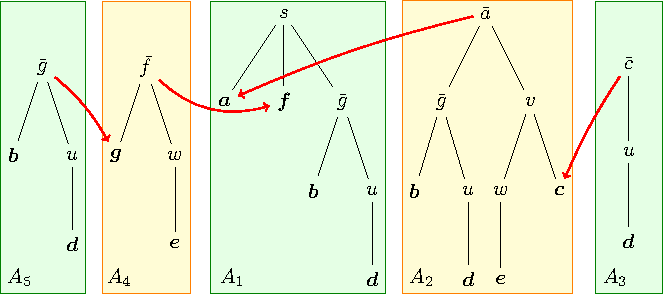
\includegraphics[scale=0.8]{diagrams/full_diagram.pdf}}
%      \caption{Your caption here.}
%    \end{subfigure}
%    \hfill
%    \begin{subfigure}[t]{0.45\textwidth}
      \centering
      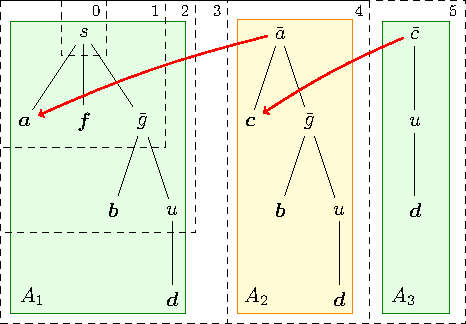
\includegraphics[scale=0.8]{diagrams/diagram.pdf}
      \caption{A dispute in five steps for the admissible (and complete) semantics justifying acceptance of the claim $s$.}
%    \end{subfigure}
%    \caption{Your caption here.}

    \label{fig:diagrams}
  \end{figure}




\section{System description, reasoning tasks}

The most obvious benefits of dispute derivations are for interactively exploring grounds for accepting claims in argumentative fashion.  %Thus, our first system implementing flexible disputes, \abaddrule (presented in~\cite{DillerGG21}), was purely interactive.  Nevertheless, automatic derivation of disputes can be a useful component of such an interactive system.
The system \flexable, implemented in the programming language \scala\footnote{\url{https://www.scala-lang.org/}}, succeeds its predecesor \abaddrule (presented in~\cite{DillerGG21}) in also having an automatic mode. Moreover, it includes several other features not relevant to the \iccma~competition, as different interactive modes, combining interactive and automatic modes, supporting approximate reasoning, as well as generating graphical outputs of disputes both in their rule as well as argument-based representation (the rule-based one being used internally by \flexable).  For further details we refer to~\cite{gor22}, the github page\footnote{\url{https://github.com/gorczyca/aba-dd-rule-based}} for \flexable, as well as a youtube overview\footnote{\url{https://www.youtube.com/watch?v=Q_28eSAjoqw}}.

As to the automatic mode of \flexable, which is what is evaluated at \iccma, this is a relatively naive implementation of a search for a dispute justifying acceptance of a set of claims.  Underlying such a search is a strategy, which consists in 1) a preference order on move types (which move types to prioritze at each step), 2) several parameters for selecting among possible rules to be made use of in a move, and 3) the option of making use of breath-first or depth-first search.  We refer to~\cite{DiGaGo22,gor22} for details.

At \iccma~\flexable participates in the subtracks of the ABA track solving the credulous acceptance problem:

\begin{itemize}
\item DC-$\sigma$ with $\sigma \in \{CO, ST\}$ (complete and stable semantics): Given an ABA framework \fr and $s \in \frL$, check whether $s$ is credulously accepted under $\sigma$.
\end{itemize}

\noindent For each of the semantics, we set the strategy to be made use of at \iccma~to be the best performing (total running time) according to our own initial experiments (also comparing to the system \abagraph~from~\cite{CravenT16}).  This ``eager'' strategy prioritizes moves from the proponent, in particular conservative forward moves (moves deducing further claims from claims already commited to); it also uses depth-first search.  For the admissible semantics, non-conservative forward moves (guessing new assumptions to be put forward) are not used. For the stable semantics, the approach we submitted to \iccma~is that which first tries to find an admissible set of assumptions congruous with the goal claim without making use of non-conservative forward moves; only when such a set of assumptions has been found this set is extended by also making use of non-conservative forward moves to obtain a stable set (when possible).  For further details we refer to~\cite{DiGaGo22,gor22} where the dispute variant for the admissible semantics is called DABF+TA and the strategy $S_2$+DFS, while for the stable semantics this is the approach that starts with the afore-mentioned combination of dispute variant and strategy for the admissible semantics (rather than using the dispute variant for the stable semantics DS+TS from the start).          

 







\bibliographystyle{IEEEtran}
\bibliography{IEEEabrv,mybib}
%\bibliographystyle{splncs04}
%\bibliography{mybib}


\end{document}
